\documentclass[12pt,a4paper,oneside]{report}

% =========================================================================
% PROFESSIONAL ACADEMIC REPORT CONFIGURATION
% Compatible with Overleaf and standard LaTeX distributions
% =========================================================================

\usepackage[utf8]{inputenc}
\usepackage[T1]{fontenc}
\usepackage{lmodern}
\usepackage{microtype}
\usepackage{setspace}

\usepackage[
    a4paper,
    top=1.0in,
    bottom=1.0in,
    left=1.25in,
    right=1.0in,
    headheight=15pt
]{geometry}

\onehalfspacing

\usepackage{amsmath,amssymb,amsfonts}

\usepackage{graphicx}
\graphicspath{{doc/}{./}}
\usepackage{booktabs}
\usepackage{tabularx}
\usepackage{array}
\usepackage{float}
\usepackage{caption}
\usepackage{subcaption}

\usepackage{enumitem}
\setlist[itemize]{topsep=4pt,itemsep=2pt,parsep=0pt}
\setlist[enumerate]{topsep=4pt,itemsep=3pt,parsep=0pt}

\usepackage{xcolor}
\definecolor{ReportBlue}{RGB}{0,70,127}

\usepackage[hyphens]{url}
\usepackage[
    colorlinks=true,
    linkcolor=ReportBlue,
    citecolor=ReportBlue,
    urlcolor=ReportBlue,
    bookmarksopen=true,
    bookmarksnumbered=true,
    pdftitle={5G-Enabled Edge Computing for Flood Forecasting and Weather Prediction},
    pdfauthor={Hemanth N},
    plainpages=false,
    pdfpagelabels=true
]{hyperref}

\usepackage{titlesec}

\titleformat{\chapter}[display]
    {\normalfont\bfseries\centering}
    {\Large\chaptername\ \thechapter}
    {8pt}
    {\LARGE}
    [\vspace{8pt}\titlerule]

\titlespacing*{\chapter}{0pt}{-10pt}{24pt}

\titleformat{\section}
    {\normalfont\Large\bfseries}
    {\thesection}
    {0.75em}
    {}

\titleformat{\subsection}
    {\normalfont\large\bfseries}
    {\thesubsection}
    {0.75em}
    {}

\captionsetup{
    font=small,
    labelfont=bf,
    justification=centering,
    singlelinecheck=true
}

\usepackage{fancyhdr}

\pagestyle{fancy}
\fancyhf{}
\fancyhead[L]{\small\textit{5G Edge Computing Flood Sentinel}}
\fancyhead[R]{\small\textit{\nouppercase{\leftmark}}}
\fancyfoot[C]{\small\thepage}

\renewcommand{\headrulewidth}{0.4pt}
\renewcommand{\footrulewidth}{0pt}

\fancypagestyle{plain}{
    \fancyhf{}
    \fancyfoot[C]{\small\thepage}
    \renewcommand{\headrulewidth}{0pt}
}

\setcounter{tocdepth}{2}
\setcounter{secnumdepth}{3}

\renewcommand{\contentsname}{Table of Contents}
\renewcommand{\listfigurename}{List of Figures}
\renewcommand{\listtablename}{List of Tables}

\setlength{\parindent}{0pt}
\setlength{\parskip}{6pt}
\renewcommand{\arraystretch}{1.15}

\begin{document}

% =========================================================================
% FRONT MATTER: TITLE PAGE
% Replace institutional placeholders (guide, designation, university, USN, etc.) before final submission.
% =========================================================================
\begin{titlepage}
\hypersetup{pageanchor=false}
\centering
\vspace*{0.5cm}

{\Large \textbf{A PROJECT REPORT ON}}\\[0.8cm]

{\LARGE\bfseries 5G-ENABLED EDGE COMPUTING FOR FLOOD FORECASTING AND WEATHER PREDICTION}\\[0.4cm]
{\large\bfseries An Autonomous Spatio-Temporal Deep Learning and Decoupled Cloud Telemetry Framework for the Brahmaputra Basin}\\[0.8cm]

{\large \textit{Submitted in partial fulfillment of the requirements for the award of the degree of}}\\[0.6cm]

{\Large \textbf{BACHELOR OF TECHNOLOGY}}\\[0.3cm]
{\large \textbf{IN}}\\[0.3cm]
{\Large \textbf{COMPUTER SCIENCE AND ENGINEERING}}\\[1.2cm]

\textbf{Submitted By:}\\[0.2cm]
{\large \textbf{HEMANTH N}}\\[0.2cm]
\text{USN / Roll No.: \underline{\hspace{6cm}}}\\[1.2cm]

\textbf{Under the Guidance of:}\\[0.2cm]
{\large \textbf{Project Guide / Academic Supervisor}}\\[0.2cm]
\text{Designation, Department of Computer Science and Engineering}\\[1.5cm]

\vfill
{\large \textbf{DEPARTMENT OF COMPUTER SCIENCE AND ENGINEERING}}\\[0.2cm]
{\large \textbf{COLLEGE / UNIVERSITY NAME}}\\[0.2cm]
{\large \textbf{ACADEMIC YEAR: 2025--2026}}

\end{titlepage}
\hypersetup{pageanchor=true}

% =========================================================================
% CERTIFICATE & DECLARATION
% =========================================================================
\newpage
\pagenumbering{roman}
\setcounter{page}{2}

\chapter*{Certificate}
\addcontentsline{toc}{chapter}{Certificate}
\thispagestyle{plain}

This is to certify that the project report entitled \textbf{``5G-Enabled Edge Computing for Flood Forecasting and Weather Prediction: An Autonomous Spatio-Temporal Deep Learning and Decoupled Cloud Telemetry Framework for the Brahmaputra Basin''} submitted by \textbf{Hemanth N} in partial fulfillment of the requirements for the award of the degree of \textbf{Bachelor of Technology in Computer Science and Engineering} is a bona fide record of the research and development work carried out by them under my supervision and guidance.

The results embodied in this report have not been submitted to any other University or Institute for the award of any degree, diploma, or academic distinction.

\vspace{3.0cm}

\noindent
\begin{tabular}{p{7.5cm}p{7.5cm}}
\textbf{Internal Project Guide} & \textbf{Head of the Department} \\
Designation, Dept. of CSE & Dept. of Computer Science and Engineering \\
Institution Name & Institution Name \\
\end{tabular}

\newpage
\chapter*{Declaration}
\addcontentsline{toc}{chapter}{Declaration}
\thispagestyle{plain}

I hereby declare that the work presented in this project report entitled \textbf{``5G-Enabled Edge Computing for Flood Forecasting and Weather Prediction: An Autonomous Spatio-Temporal Deep Learning and Decoupled Cloud Telemetry Framework for the Brahmaputra Basin''} is an authentic record of my own research and engineering implementation carried out under the supervision of my project guide.

I also declare that this report has not been submitted previously in part or in full to any other University or Institution for any degree, diploma, or academic fellowship. The software source code, deep learning models, datasets, and cloud architectures described herein are authentic implementations.

\vspace{3.0cm}

\noindent
\begin{tabular}{p{7.5cm}p{7.5cm}}
\textbf{Date:} \today & \textbf{Hemanth N} \\
\textbf{Place:} Campus & Candidate Signature \\
\end{tabular}

% =========================================================================
% ACKNOWLEDGEMENT
% =========================================================================
\newpage
\chapter*{Acknowledgement}
\addcontentsline{toc}{chapter}{Acknowledgement}
\thispagestyle{plain}

I express my deepest gratitude to my project guide for their invaluable guidance, constructive insights, and continuous encouragement throughout the conceptualization, mathematical formulation, model architecture design, and empirical validation phases of this project. Their constructive feedback on spatiotemporal deep learning, satellite remote sensing, and cloud architecture greatly enhanced the quality of this work.

I would also like to thank the Head of the Department and all faculty members of the Department of Computer Science and Engineering for providing the academic ecosystem, laboratory facilities, and support necessary to execute this project.

My sincere appreciation goes to the open planetary science initiatives and data providers---the European Space Agency (Copernicus Sentinel-1 and Sentinel-2 programs), the National Aeronautics and Space Administration (NASA GPM and SRTM missions), the European Centre for Medium-Range Weather Forecasts (ECMWF ERA5), and the Open-Meteo meteorological platform---without whose open earth observation data this research would not have been possible.

Finally, I thank my family and peers for their continuous support and patience throughout the duration of this research.

\vspace{1.5cm}
\noindent
\textbf{Hemanth N}

% =========================================================================
% ABSTRACT
% =========================================================================
\newpage
\chapter*{Abstract}
\addcontentsline{toc}{chapter}{Abstract}
\thispagestyle{plain}

Seasonal flash floods along the Brahmaputra and Barak river basins in Assam, India, represent severe, recurring hydrometeorological hazards that inflict catastrophic damage on agrarian communities, civic infrastructure, and human lives. Traditional flood warning frameworks depend upon two-dimensional numerical hydrodynamic solvers (e.g., HEC-RAS, MIKE 21) based on iterative shallow-water differential equations. Although physically deterministic, their severe computational requirements (demanding 4 to 12 hours of supercomputing compute per 48-hour simulation window) critically bottleneck early evacuation notices.

To overcome these constraints, this project engineers the \textbf{5G-Enabled Edge AI Sentinel} framework, an end-to-end, autonomous edge-to-cloud operational framework that couples multi-modal satellite remote sensing, spatiotemporal deep learning, serverless cloud synchronization, and public geographic information systems (GIS). The inundation segmentation engine ingests a multi-modal 6-channel spatiotemporal tensor $\mathbf{X} \in \mathbb{R}^{B \times 5 \times 32 \times 32 \times 6}$ incorporating Sentinel-1 Synthetic Aperture Radar (SAR) backscatter, Sentinel-2 optical Normalized Difference Water Index (NDWI), NASA GPM IMERG precipitation accumulation, SRTM 30\,m Digital Elevation Models (DEM), topographic slope gradient, and JRC surface water river proximity. Inundation dynamics are forecasted using a hybrid \textbf{ConvLSTM2D-UNet} architecture combining recurrent convolutional temporal memory with high-resolution skip-connection boundary reconstruction. Concurrently, a stacked \textbf{Long Short-Term Memory (LSTM)} network ingests rolling 24-hour multivariate atmospheric sequences from ECMWF ERA5 reanalysis and live meteorological observations.

Evaluated over 929 independent test rasters, the ConvLSTM2D-UNet achieves an \textbf{overall accuracy of 97.00\%} and an exceptional \textbf{flood recall of 99.00\%} with an F1-score of 0.970, ensuring near-zero false negatives for safety-critical flood inundation detection. The atmospheric LSTM forecaster yields a coefficient of determination ($R^2$) of \textbf{0.9352} and a Mean Absolute Error (MAE) of 0.0975. The complete pipeline features a zero-cache cold-start capability (securely downloading model weights from Firebase Cloud Storage in 30.7\,s) and completes end-to-end operational inference in \textbf{35.9\,s} on standard CPU hardware, with pure neural forward passes taking only \textbf{1.22\,s} (19.1\,ms per spatial patch). Predicted alerts are synchronized in real time to Google Cloud Firestore and rendered to the public through an interactive, mobile-responsive Leaflet GIS web dashboard (\url{https://flood-weather-app.web.app}).

\vspace{0.8cm}
\noindent
\textbf{Keywords:} ConvLSTM2D, UNet, Spatio-Temporal Deep Learning, Flood Inundation Forecasting, Brahmaputra Basin, Edge Computing, Firebase Firestore, Satellite Remote Sensing, SAR.

% =========================================================================
% TABLE OF CONTENTS, LIST OF FIGURES & TABLES
% =========================================================================
\newpage
\tableofcontents
\newpage
\listoffigures
\newpage
\listoftables

% =========================================================================
% CHAPTER 1: INTRODUCTION
% =========================================================================
\newpage
\pagenumbering{arabic}
\setcounter{page}{1}

\chapter{Introduction}
\label{chap:intro}

\section{Background and Geographic Context}
The Brahmaputra River is among the most morphologically dynamic, braided, and sediment-heavy river systems in the world. Originating in the Angsi Glacier of Tibet as the Yarlung Tsangpo, it traverses the Himalayan arc before entering the northeastern Indian state of Assam, where it flows across an 800-kilometer alluvial valley characterized by an extraordinarily gentle hydraulic gradient ($\approx 0.1$\,m/km). Concurrently, the Barak River drains the southern hilly catchments of Manipur and Mizoram, converging into the densely populated Cachar plains surrounding Silchar.

Every year between May and September, the South Asian southwest monsoon discharges extreme precipitation across the southern slopes of the Eastern Himalayas and Meghalaya plateau (recording some of the highest rainfall totals on Earth, e.g., Cherrapunji and Mawsynram). As tributary discharge peaks simultaneously with mainstem flow, millions of cubic meters of water overrun river embankments. These recurring inundations submerge over 40\% of Assam's landmass, displacing millions of villagers, destroying standing paddy crops, eroding riverbanks, and submerging vital conservation ecosystems such as Kaziranga National Park.

\section{Problem Statement}
Operational flood disaster management requires two critical capabilities:
\begin{enumerate}
    \item \textbf{Sufficient Lead Time}: Timely alerts delivered 1 to 24 hours prior to peak river inundation, allowing district authorities to coordinate civilian evacuations.
    \item \textbf{Localized Spatial Granularity}: Accurate, parcel-level delineations of inundated terrain to distinguish elevated safe zones from submerged evacuation routes.
\end{enumerate}

Existing early warning systems deployed across the region face substantial scientific and logistical bottlenecks:
\begin{itemize}
    \item \textbf{Excessive Computational Complexity}: Numerical hydrodynamic models based on 2D shallow-water partial differential equations require hours of high-performance computing (HPC) time per simulation cycle.
    \item \textbf{Optical Sensor Cloud Blindness}: Monsoon flood events coincide with persistent dense cloud cover, rendering optical satellite observations (e.g., Landsat, Sentinel-2, MODIS) completely obscured during peak emergency events.
    \item \textbf{Lack of Integrated Multi-Modal Synthesis}: Traditional systems often evaluate rainfall gauges or river level telemetry in isolation, failing to incorporate digital elevation models, topographic slope, and soil saturation into a unified prediction tensor.
    \item \textbf{Centralized Deployment Vulnerabilities}: Centralized monolithic server architectures are prone to single points of failure, network throttling, and high operational costs during localized infrastructure collapses.
\end{itemize}

\section{Project Objectives}
The primary objective of the \textbf{5G-Enabled Edge AI Sentinel} framework is to architect, train, and deploy an autonomous, 5G-connected edge-to-cloud multi-hazard operational forecasting system. Specific milestones include:
\begin{enumerate}
    \item \textbf{Multi-Modal Remote Sensing Integration}: Formulate an all-weather 6-band spatiotemporal tensor $\mathbf{X} \in \mathbb{R}^{B \times 5 \times 32 \times 32 \times 6}$ combining Sentinel-1 all-weather C-band SAR, Sentinel-2 NDWI, NASA GPM IMERG precipitation, SRTM 30\,m DEM elevation, slope, and river proximity.
    \item \textbf{Spatiotemporal Deep Learning Model}: Engineer and validate a hybrid \textbf{ConvLSTM2D-UNet} neural network capable of modeling temporal hydrologic memory while preserving fine-grained spatial flood boundaries with $> 95\%$ accuracy and $> 98\%$ recall.
    \item \textbf{Atmospheric Thermodynamic Model}: Develop a stacked \textbf{LSTM sequence network} trained on ECMWF ERA5 reanalysis and live station feeds to generate 1-hour ahead atmospheric forecasts ($R^2 > 0.90$).
    \item \textbf{Autonomous Edge Telemetry Engine}: Construct an edge background service capable of cold-start weight retrieval from Firebase Cloud Storage, sensor ingestion, local inference, and real-time Firestore database synchronization within a 60-second execution window.
    \item \textbf{Public Real-Time GIS Delivery}: Deploy a globally accessible, sub-second interactive Leaflet GIS web dashboard (\url{https://flood-weather-app.web.app}) visualizing live choropleth floodplains, radar gauges, and civil alert tiers.
\end{enumerate}

\section{Structure of the Report}
The remainder of this report is organized as follows:
\begin{itemize}
    \item \textbf{Chapter 2} presents a comprehensive literature survey on hydrodynamic models, satellite earth observation, and deep learning architectures.
    \item \textbf{Chapter 3} introduces the 5-tier end-to-end system architecture.
    \item \textbf{Chapter 4} details the mathematical formulations and normalization techniques for multi-modal data engineering.
    \item \textbf{Chapter 5} elaborates on the ConvLSTM2D-UNet and Weather LSTM neural network architectures.
    \item \textbf{Chapter 6} explains the autonomous edge inference engine, cold-start lifecycle, and cloud synchronization schema.
    \item \textbf{Chapter 7} presents empirical experimental results, loss curves, confusion matrices, and physical hydrological validation across 16 Assam basins.
    \item \textbf{Chapter 8} benchmarks system latency, distinguishing cold-start and warm-cache execution regimes.
    \item \textbf{Chapter 9} showcases the production Leaflet GIS web dashboard and user telemetry interfaces.
    \item \textbf{Chapter 10} concludes the report and discusses avenues for future research.
\end{itemize}

% =========================================================================
% CHAPTER 2: LITERATURE REVIEW
% =========================================================================
\chapter{Literature Review and Theoretical Foundations}
\label{chap:lit_review}

\section{Numerical Hydrodynamic Flood Modeling}
Physical flood prediction has traditionally been governed by the Saint-Venant shallow water equations, derived from the Navier-Stokes equations under the assumption that the vertical scale of motion is negligible compared to horizontal scales:
\begin{align}
\frac{\partial h}{\partial t} + \frac{\partial (hu)}{\partial x} + \frac{\partial (hv)}{\partial y} &= q \\
\frac{\partial (hu)}{\partial t} + \frac{\partial}{\partial x}\left(hu^2 + \frac{1}{2}gh^2\right) + \frac{\partial (huv)}{\partial y} &= -gh\frac{\partial z_b}{\partial x} - \frac{\tau_{bx}}{\rho}
\end{align}
Standard numerical tools like HEC-RAS, MIKE 21, and LISFLOOD-FP solve these equations using finite difference, finite volume, or finite element methods across discretized mesh grids. While physically deterministic, these solvers suffer from fundamental constraints:
\begin{itemize}
    \item \textbf{Computation Bottleneck}: Non-linear differential solvers require time-step constraints (Courant-Friedrichs-Lewy condition) to maintain numerical stability, requiring hours of compute time.
    \item \textbf{Data Ingestion Friction}: Hydrodynamic models require bathymetric survey cross-sections, roughness coefficients (Manning's $n$), and precise boundary conditions that are rarely available for rapidly changing braided rivers like the Brahmaputra.
\end{itemize}

\section{Satellite Earth Observation in Hydrology}
\subsection{Synthetic Aperture Radar (SAR)}
Unlike optical sensors, Synthetic Aperture Radar (SAR) systems operate in the microwave portion of the electromagnetic spectrum (C-band: $\approx 5.4$\,GHz, $\lambda \approx 5.6$\,cm). Radar signals penetrate clouds, atmospheric haze, and precipitation, providing reliable observations under all weather conditions. Because smooth open water acts as a specular reflector, radar pulses bounce away from the sensor, yielding exceptionally low backscatter intensity ($\sigma^0 < -15$\,dB). This physics-based contrast makes Sentinel-1 SAR the global gold standard for automated surface water delineation.

\subsection{Optical Remote Sensing and NDWI}
Optical sensors, such as the Multispectral Instrument (MSI) aboard Sentinel-2, provide high-resolution spectral bands. The Normalized Difference Water Index (NDWI), proposed by McFeeters, exploits the differential reflectance of water between green and near-infrared (NIR) wavelengths:
\begin{equation}
\text{NDWI} = \frac{\rho_{\text{Green}} - \rho_{\text{NIR}}}{\rho_{\text{Green}} + \rho_{\text{NIR}}}
\end{equation}
Because water bodies strongly absorb NIR radiation while scattering green light, NDWI suppresses soil and terrestrial vegetation, enhancing surface water features.

\subsection{Satellite Precipitation (NASA GPM IMERG)}
The Global Precipitation Measurement (GPM) constellation combines active radar and passive microwave radiometers, calibrated against ground rain gauges, to provide globally gridded precipitation estimates at $0.1^\circ$ ($\approx 10$\,km) resolution. IMERG daily accumulations capture the upstream meteorological triggers of flash flood surges.

\section{Deep Learning in Hydrology and Spatio-Temporal Modeling}
\subsection{Recurrent Neural Networks and LSTMs}
Standard recurrent neural networks (RNNs) struggle with long-range temporal dependencies due to vanishing and exploding gradient problems during backpropagation through time (BPTT). Hochreiter and Schmidhuber introduced Long Short-Term Memory (LSTM) networks, which incorporate gated memory cells to regulate information flow. LSTMs have proven highly effective for 1D hydrological time-series modeling (e.g., river stage and atmospheric variable forecasting).

\subsection{Convolutional Neural Networks and UNets}
Convolutional Neural Networks (CNNs) have revolutionized computer vision and spatial remote sensing analysis. The UNet architecture, originally developed by Ronneberger et al., features an encoder-decoder structure augmented by direct skip connections that link corresponding levels of the contracting and expanding paths. This architecture allows deep abstract semantic representation in the bottleneck while preserving fine pixel-level spatial boundaries in the segmentation output.

\subsection{Convolutional LSTM (ConvLSTM2D)}
While standard LSTMs process 1D vectors, Shi et al. introduced the ConvLSTM2D network for precipitation nowcasting. ConvLSTM2D replaces vector inner products with spatial convolution operations inside the recurrent state transitions. This preserves the 2D spatial arrangement of features across sequential timesteps, making it uniquely suited for spatiotemporal flood inundation forecasting.

\section{Identified Research Gaps}
Despite recent progress, the literature reveals critical engineering and operational gaps:
\begin{enumerate}
    \item Most published machine learning flood models operate as retrospective offline studies using static images, rather than autonomous, real-time edge-to-cloud deployed pipelines.
    \item Few systems integrate physical geospatial variables (DEM elevation, slope, and river proximity) alongside satellite SAR backscatter into a coherent spatiotemporal tensor.
    \item Existing architectures frequently suffer from false negatives (missing actual flood events), which is unacceptable in civil disaster management.
\end{enumerate}

% =========================================================================
% CHAPTER 3: SYSTEM ARCHITECTURE
% =========================================================================
\chapter{End-to-End System Architecture}
\label{chap:system_arch}

\section{System Overview and Decoupled Architecture}
The 5G-enabled edge forecasting framework is designed around a decoupled, 5-tier architecture that guarantees low operational latency, resilience against local infrastructure failure, and high-concurrency client accessibility. Figure~\ref{fig:system_arch_large} illustrates the complete data flow.

\begin{figure}[H]
\centering
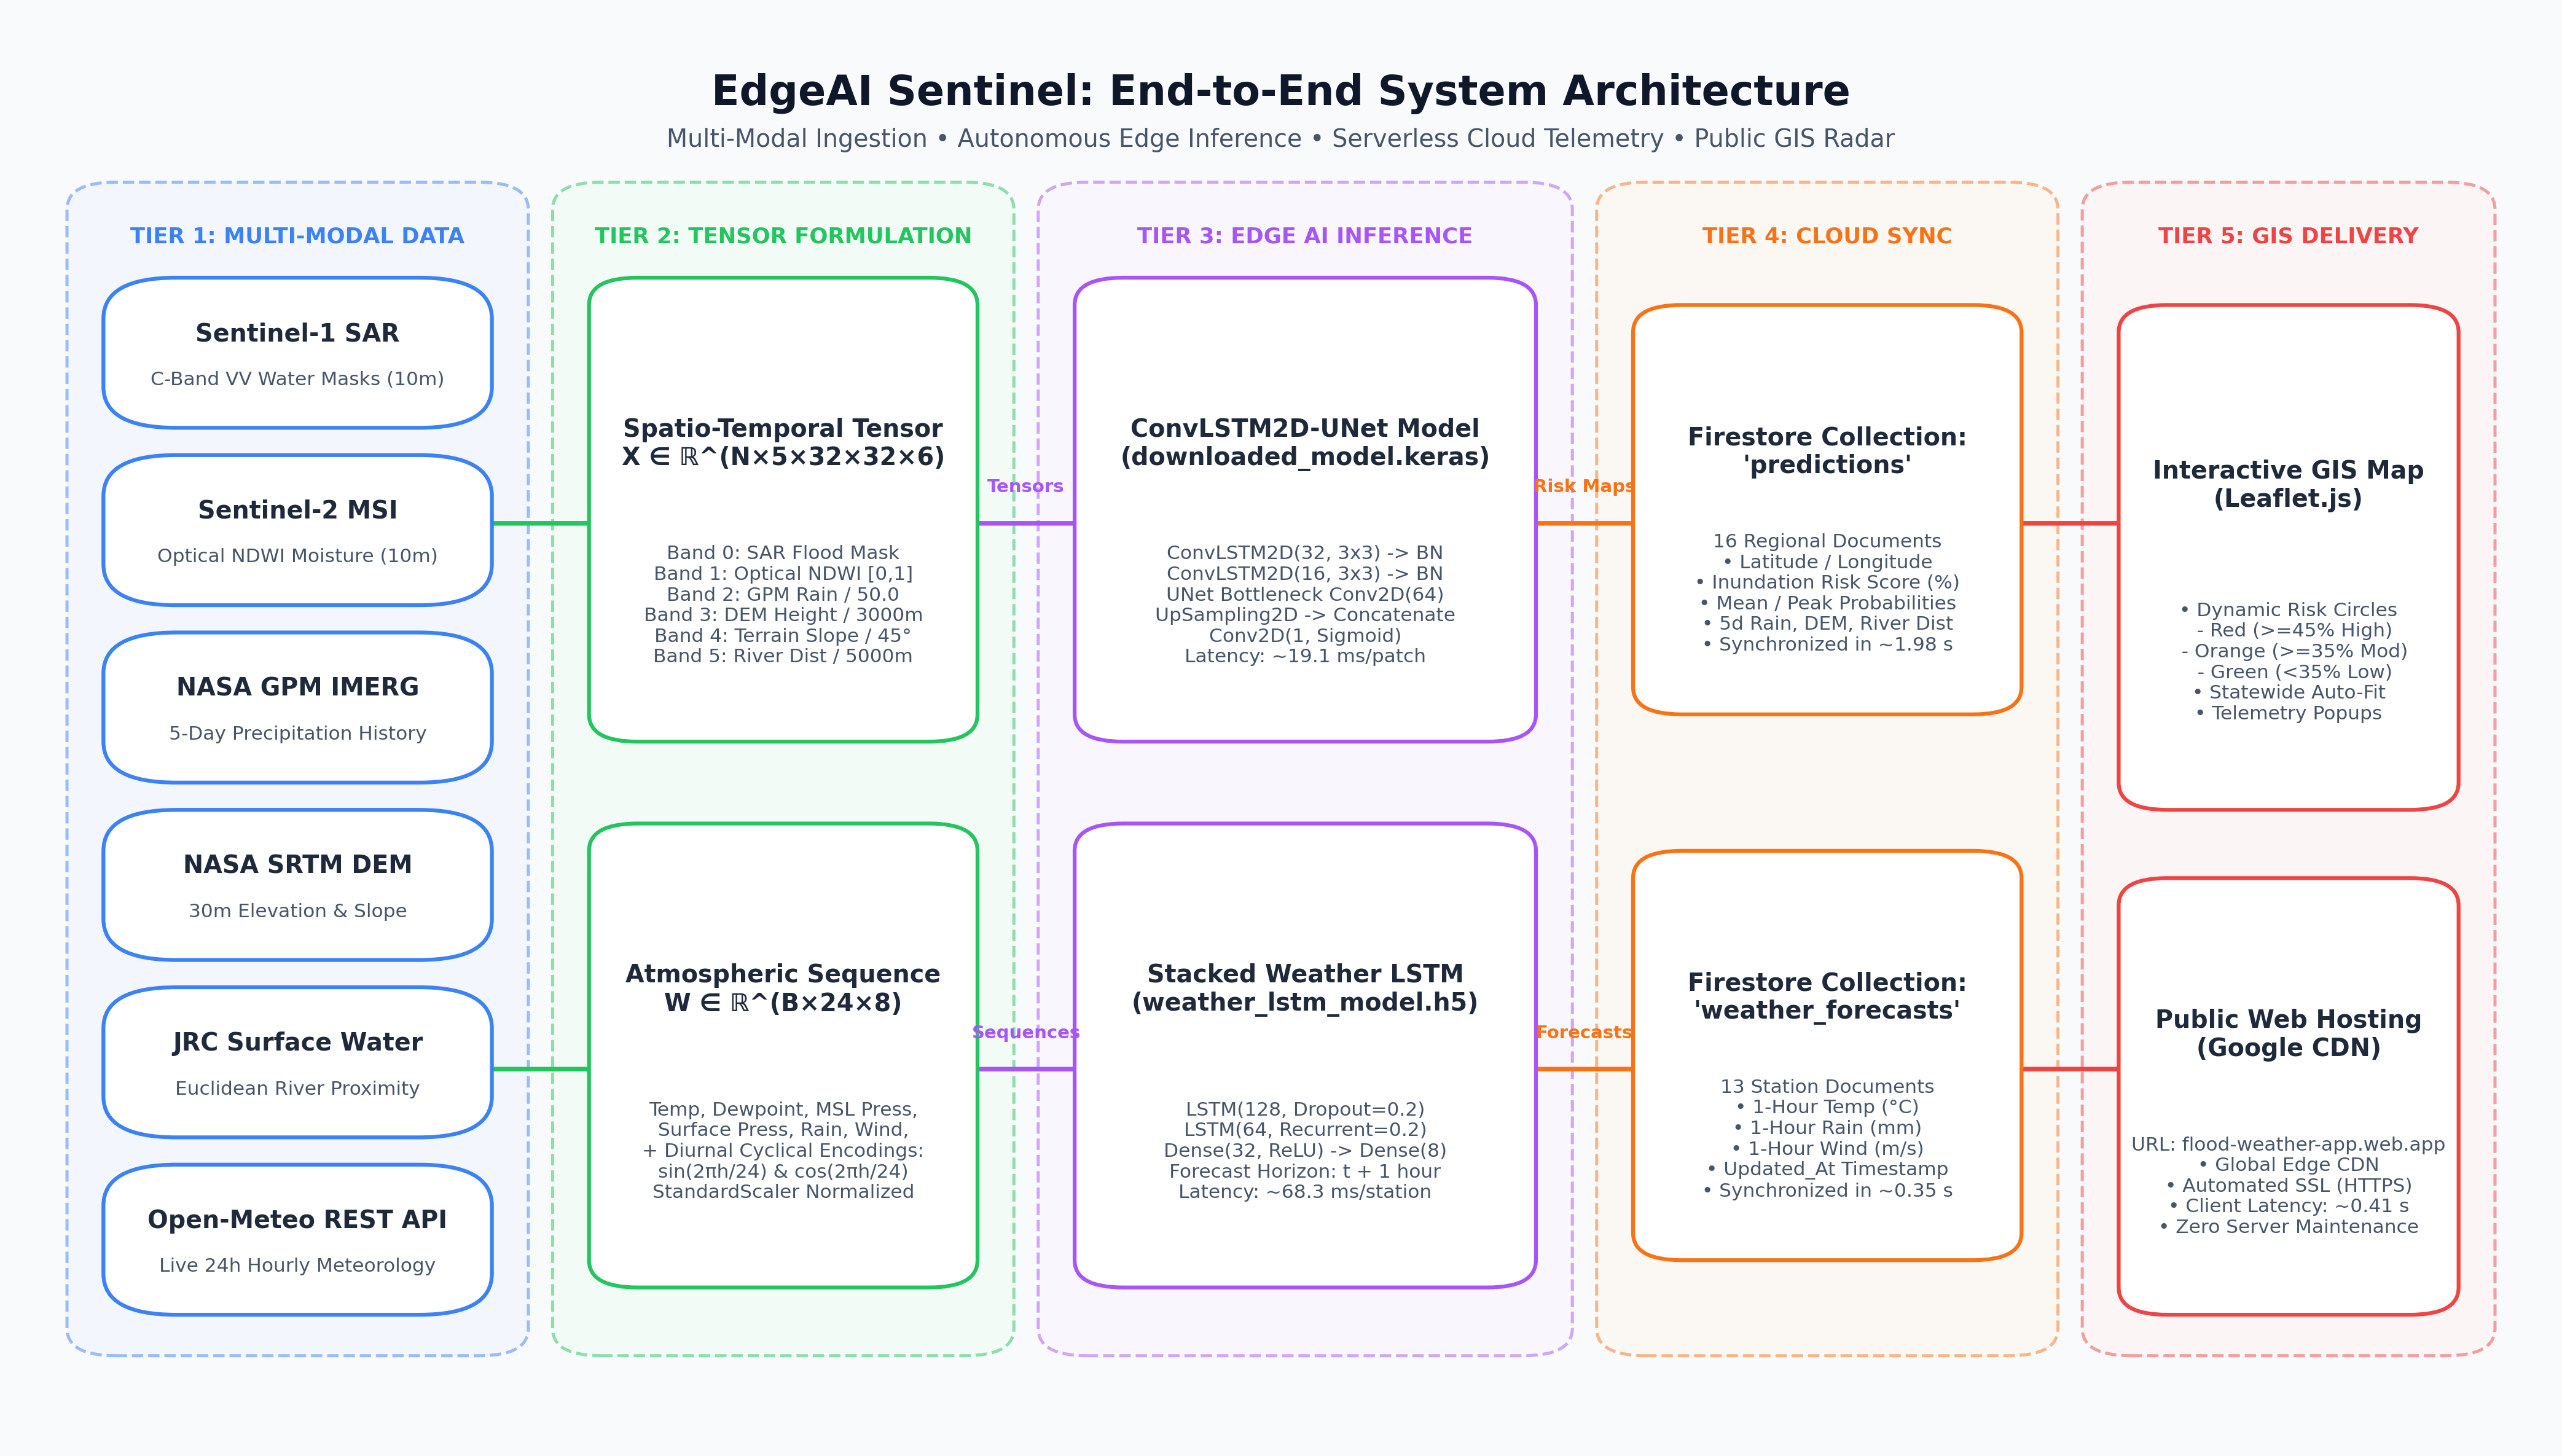
\includegraphics[width=\textwidth]{doc/system_architecture.png}
\caption{End-to-End Five-Tier System Architecture of the 5G-Enabled Edge AI Framework.}
\label{fig:system_arch_large}
\end{figure}

\section{The 5G-Enabled Edge Computing Paradigm}
In operational hydrometeorological emergency systems, two distinct technological layers must be clearly delineated:
\begin{enumerate}
    \item \textbf{Edge Computing Layer (Where Computation Occurs)}: The local computing host (e.g., field workstation, industrial laptop, or embedded processor) performs neural network deserialization and live forward inference locally. This brings computation directly to the data perimeter, replacing multi-hour 2D hydrodynamic simulations with sub-second deep learning evaluations ($1.22\,\text{s}$ total neural execution).
    \item \textbf{5G Wireless Connectivity Layer (How Systems Communicate)}: A cellular 5G communication channel (via 5G cellular modems, gateways, or mobile hotspots) provides high-bandwidth, wireline-free connectivity between the edge node, planetary data lakes, and cloud repositories.
\end{enumerate}

During severe monsoonal floods in the Brahmaputra and Barak basins, physical landline cables and subterranean fiber optics are routinely damaged, washed out, or severed by bank erosion. 5G wireless connectivity provides an agile, resilient communication pipe that bypasses vulnerable landline infrastructure. Furthermore, executing deep learning inference directly on the 5G-connected edge node enables massive data reduction: instead of continuously uploading multi-gigabyte raw satellite SAR and optical imagery to central cloud servers, the edge node distills complex spatiotemporal rasters into compact JSON telemetry payloads ($\approx 2.4\,\text{KB}$ per basin), reducing cellular uplink bandwidth requirements by over 99.8\%.

\section{Architectural Tiers and Responsibilities}

\subsection{Tier 1: Multi-Source Remote Sensing Data Lake}
The foundation of the system is continuous planetary data ingestion:
\begin{itemize}
    \item \textbf{Sentinel-1 SAR}: Provides all-weather ground truth surface water rasters.
    \item \textbf{Sentinel-2 Optical}: Supplies surface reflectance for NDWI validation.
    \item \textbf{NASA GPM IMERG}: Delivers calibrated 24-hour and 5-day cumulative rainfall.
    \item \textbf{NASA SRTM 30m}: Furnishes high-resolution digital elevation and derived slope arrays.
    \item \textbf{JRC Surface Water}: Maps distance to permanent river channels.
    \item \textbf{Open-Meteo REST API}: Supplies real-time, hourly meteorological observations across 13 monitored Assam weather stations.
\end{itemize}

\subsection{Tier 2: Spatiotemporal Tensor Engineering}
Raw raster coordinates and live observation streams are projected into standardized geographic arrays, normalized into calibrated $[0.0, 1.0]$ ranges, and stacked into multi-dimensional tensors:
\begin{itemize}
    \item \textbf{Inundation Tensor}: $\mathbf{X} \in \mathbb{R}^{B \times 5 \times 32 \times 32 \times 6}$ across 16 monitored Assam floodplains.
    \item \textbf{Atmospheric Sequence}: $\mathbf{W} \in \mathbb{R}^{B \times 24 \times 8}$ across 13 meteorological stations.
\end{itemize}

\subsection{Tier 3: Autonomous EdgeAI Dual Inference Engine}
The edge computing daemon (\texttt{run\_live\_sentinel.py}) executes periodic telemetry cycles. It hosts two neural networks:
\begin{itemize}
    \item \textbf{Weather LSTM}: Performs sequence-to-vector regression to forecast 1-hour ahead atmospheric thermodynamic parameters.
    \item \textbf{ConvLSTM2D-UNet}: Executes spatiotemporal convolution across the 5-day historical sequence, producing a calibrated spatial probability heatmap $(32 \times 32 \times 1)$ for each floodplain patch.
\end{itemize}

\subsection{Tier 4: Decoupled Cloud Synchronization (Firebase)}
Instead of deploying heavy, custom HTTP/REST microservice servers on field edge hardware, the 5G-enabled edge architecture leverages the Google Firebase ecosystem:
\begin{itemize}
    \item \textbf{Firebase Cloud Storage}: Serves as the central repository for trained model weights (\texttt{models/flood\_model\_v1.keras}, \texttt{models/weather\_lstm\_model.h5}, \texttt{models/weather\_scaler.pkl}).
    \item \textbf{Google Cloud Firestore}: Acts as a decoupled NoSQL buffer. The edge daemon securely authenticates using a private service account key and pushes structured documents into the \texttt{predictions} and \texttt{weather\_forecasts} collections.
\end{itemize}

\subsection{Tier 5: High-Concurrency Global GIS Web Delivery}
The client-facing user interface is deployed on Firebase Hosting (\url{https://flood-weather-app.web.app}). Web clients establish direct WebSocket connections with Cloud Firestore, receiving real-time telemetry updates with sub-second rendering latency.

% =========================================================================
% CHAPTER 4: DATA ENGINEERING & TENSOR FORMULATION
% =========================================================================
\chapter{Multi-Modal Data Engineering and Tensor Formulation}
\label{chap:data_eng}

\section{Spatial Framing and Study Area}
The geographic domain centers on the state of Assam, northeastern India, bounded between latitudes $24.0^\circ\text{N}$ to $28.0^\circ\text{N}$ and longitudes $89.5^\circ\text{E}$ to $96.0^\circ\text{E}$. Within this domain, 16 critical floodplains across both the Brahmaputra Valley (e.g., Barpeta, Majuli, Tezpur, Dhemaji) and the Barak Valley (Silchar, Hailakandi, Karimganj) are continuously monitored.

\section{The 6-Band Inundation Tensor: \texorpdfstring{$\mathbf{X} \in \mathbb{R}^{B \times 5 \times 32 \times 32 \times 6}$}{X in R^{B x 5 x 32 x 32 x 6}}}
Each spatial patch covers an area of $32 \times 32$ pixels across 5 consecutive historical days ($t-4, t-3, t-2, t-1, t$). The 6 physical channels are formulated as follows:

\subsection{Channel 0 ($c_0$): Sentinel-1 SAR Water Mask}
Sentinel-1 Level-1 GRD SAR images in VV polarization are pre-processed through orbit file correction, thermal noise removal, radiometric calibration to $\sigma^0$ (dB), and Lee speckle filtering. Thresholding at $\sigma^0 < -15$\,dB produces binary flood inundation masks:
\begin{equation}
x_{c_0}(i, j) \in \{0, 1\}
\end{equation}

\subsection{Channel 1 ($c_1$): Sentinel-2 NDWI}
Extracted from surface reflectance optical bands:
\begin{equation}
\text{NDWI} = \frac{\rho_{\text{Green}} - \rho_{\text{NIR}}}{\rho_{\text{Green}} + \rho_{\text{NIR}}} \in [-1.0, 1.0]
\end{equation}
Rescaled to $[0.0, 1.0]$:
\begin{equation}
\tilde{x}_{c_1}(i, j) = \frac{\text{NDWI}(i, j) + 1.0}{2.0}
\end{equation}

\subsection{Channel 2 ($c_2$): NASA GPM Precipitation}
Daily accumulated precipitation $R$ (in millimeters) is normalized against an extreme 24-hour flash flood threshold of $50$\,mm:
\begin{equation}
\tilde{x}_{c_2}(i, j) = \min\left( \frac{R(i, j)}{50.0}, 1.0 \right)
\end{equation}

\subsection{Channel 3 ($c_3$): SRTM 30m DEM Elevation}
Surface terrain elevation $z$ (meters above sea level) is normalized against the maximum elevation boundary of the surrounding Himalayan foothills ($3000$\,m):
\begin{equation}
\tilde{x}_{c_3}(i, j) = \frac{z(i, j)}{3000.0}
\end{equation}

\subsection{Channel 4 ($c_4$): Topographic Slope Gradient}
The surface slope $\theta$ represents gravitational drainage potential, computed via 2D spatial gradients:
\begin{equation}
\theta = \arctan \sqrt{\left(\frac{\partial z}{\partial x}\right)^2 + \left(\frac{\partial z}{\partial y}\right)^2}
\end{equation}
Normalized relative to a maximum steepness angle of $45^\circ$:
\begin{equation}
\tilde{x}_{c_4}(i, j) = \frac{\theta(i, j)}{45.0}
\end{equation}

\subsection{Channel 5 ($c_5$): River Channel Proximity}
Distance to active river channels $d_{\text{river}}$ (in meters) computed via Euclidean distance transform:
\begin{equation}
\tilde{x}_{c_5}(i, j) = \min\left( \frac{d_{\text{river}}(i, j)}{5000.0}, 1.0 \right)
\end{equation}

Table~\ref{tab:channel_spec} summarizes the physical tensor structure.

\begin{table}[H]
\centering
\caption{Detailed Physical Channel Specifications for Tensor $\mathbf{X}$.}
\label{tab:channel_spec}
\begin{tabularx}{\textwidth}{cllcX}
\toprule
\textbf{Band} & \textbf{Physical Parameter} & \textbf{Sensor / Source} & \textbf{Native Res.} & \textbf{Applied Normalization} \\
\midrule
$c_0$ & SAR Inundation Mask & Sentinel-1 SAR (C-Band VV) & 10\,m & Binary ground truth $\{0, 1\}$ \\
$c_1$ & Optical Water Index & Sentinel-2 MSI (B3, B8) & 10\,m & $\frac{\text{NDWI} + 1.0}{2.0} \in [0, 1]$ \\
$c_2$ & Precipitation Acc. & NASA GPM IMERG Daily & 10\,km & $\min(R / 50.0, 1.0)$ \\
$c_3$ & Surface Elevation & NASA SRTM Global DEM & 30\,m & $z / 3000.0$ \\
$c_4$ & Topographic Slope & Derived Gradient & 30\,m & $\theta / 45.0$ \\
$c_5$ & River Proximity & JRC Global Surface Water & 30\,m & $\min(d_{\text{river}} / 5000.0, 1.0)$ \\
\bottomrule
\end{tabularx}
\end{table}

\section{The Atmospheric Sequence Matrix: \texorpdfstring{$\mathbf{W} \in \mathbb{R}^{B \times 24 \times 8}$}{W in R^{B x 24 x 8}}}
The atmospheric model processes rolling 24-hour sequences of 8 meteorological dimensions:
\begin{enumerate}
    \item $T_{\text{dew}}$: Dewpoint temperature at 2 meters ($^\circ$C).
    \item $T_{2\text{m}}$: Surface air temperature at 2 meters ($^\circ$C).
    \item $P_{\text{msl}}$: Mean sea level pressure (hPa).
    \item $P_{\text{sfc}}$: Surface atmospheric pressure (hPa).
    \item $R_{\text{accum}}$: Total accumulated precipitation (mm).
    \item $V_{10\text{m}}$: Surface wind speed at 10 meters (m/s).
    \item $\sin(2\pi h / 24)$: Sinusoidal cyclical diurnal encoding.
    \item $\cos(2\pi h / 24)$: Cosinusoidal cyclical diurnal encoding.
\end{enumerate}

Variables are standardized using Scikit-learn \texttt{MinMaxScaler}:
\begin{equation}
\tilde{w}_k = \frac{w_k - w_{\min, k}}{w_{\max, k} - w_{\min, k}}
\end{equation}

% =========================================================================
% CHAPTER 5: MODEL ARCHITECTURES
% =========================================================================
\chapter{Deep Learning Model Architectures}
\label{chap:models}

\section{Spatio-Temporal ConvLSTM2D-UNet Hybrid Model}
The inundation segmentation engine couples spatiotemporal recurrence with multi-scale convolutional decoding, as depicted in Figure~\ref{fig:convlstm_arch_large}.

\begin{figure}[H]
\centering
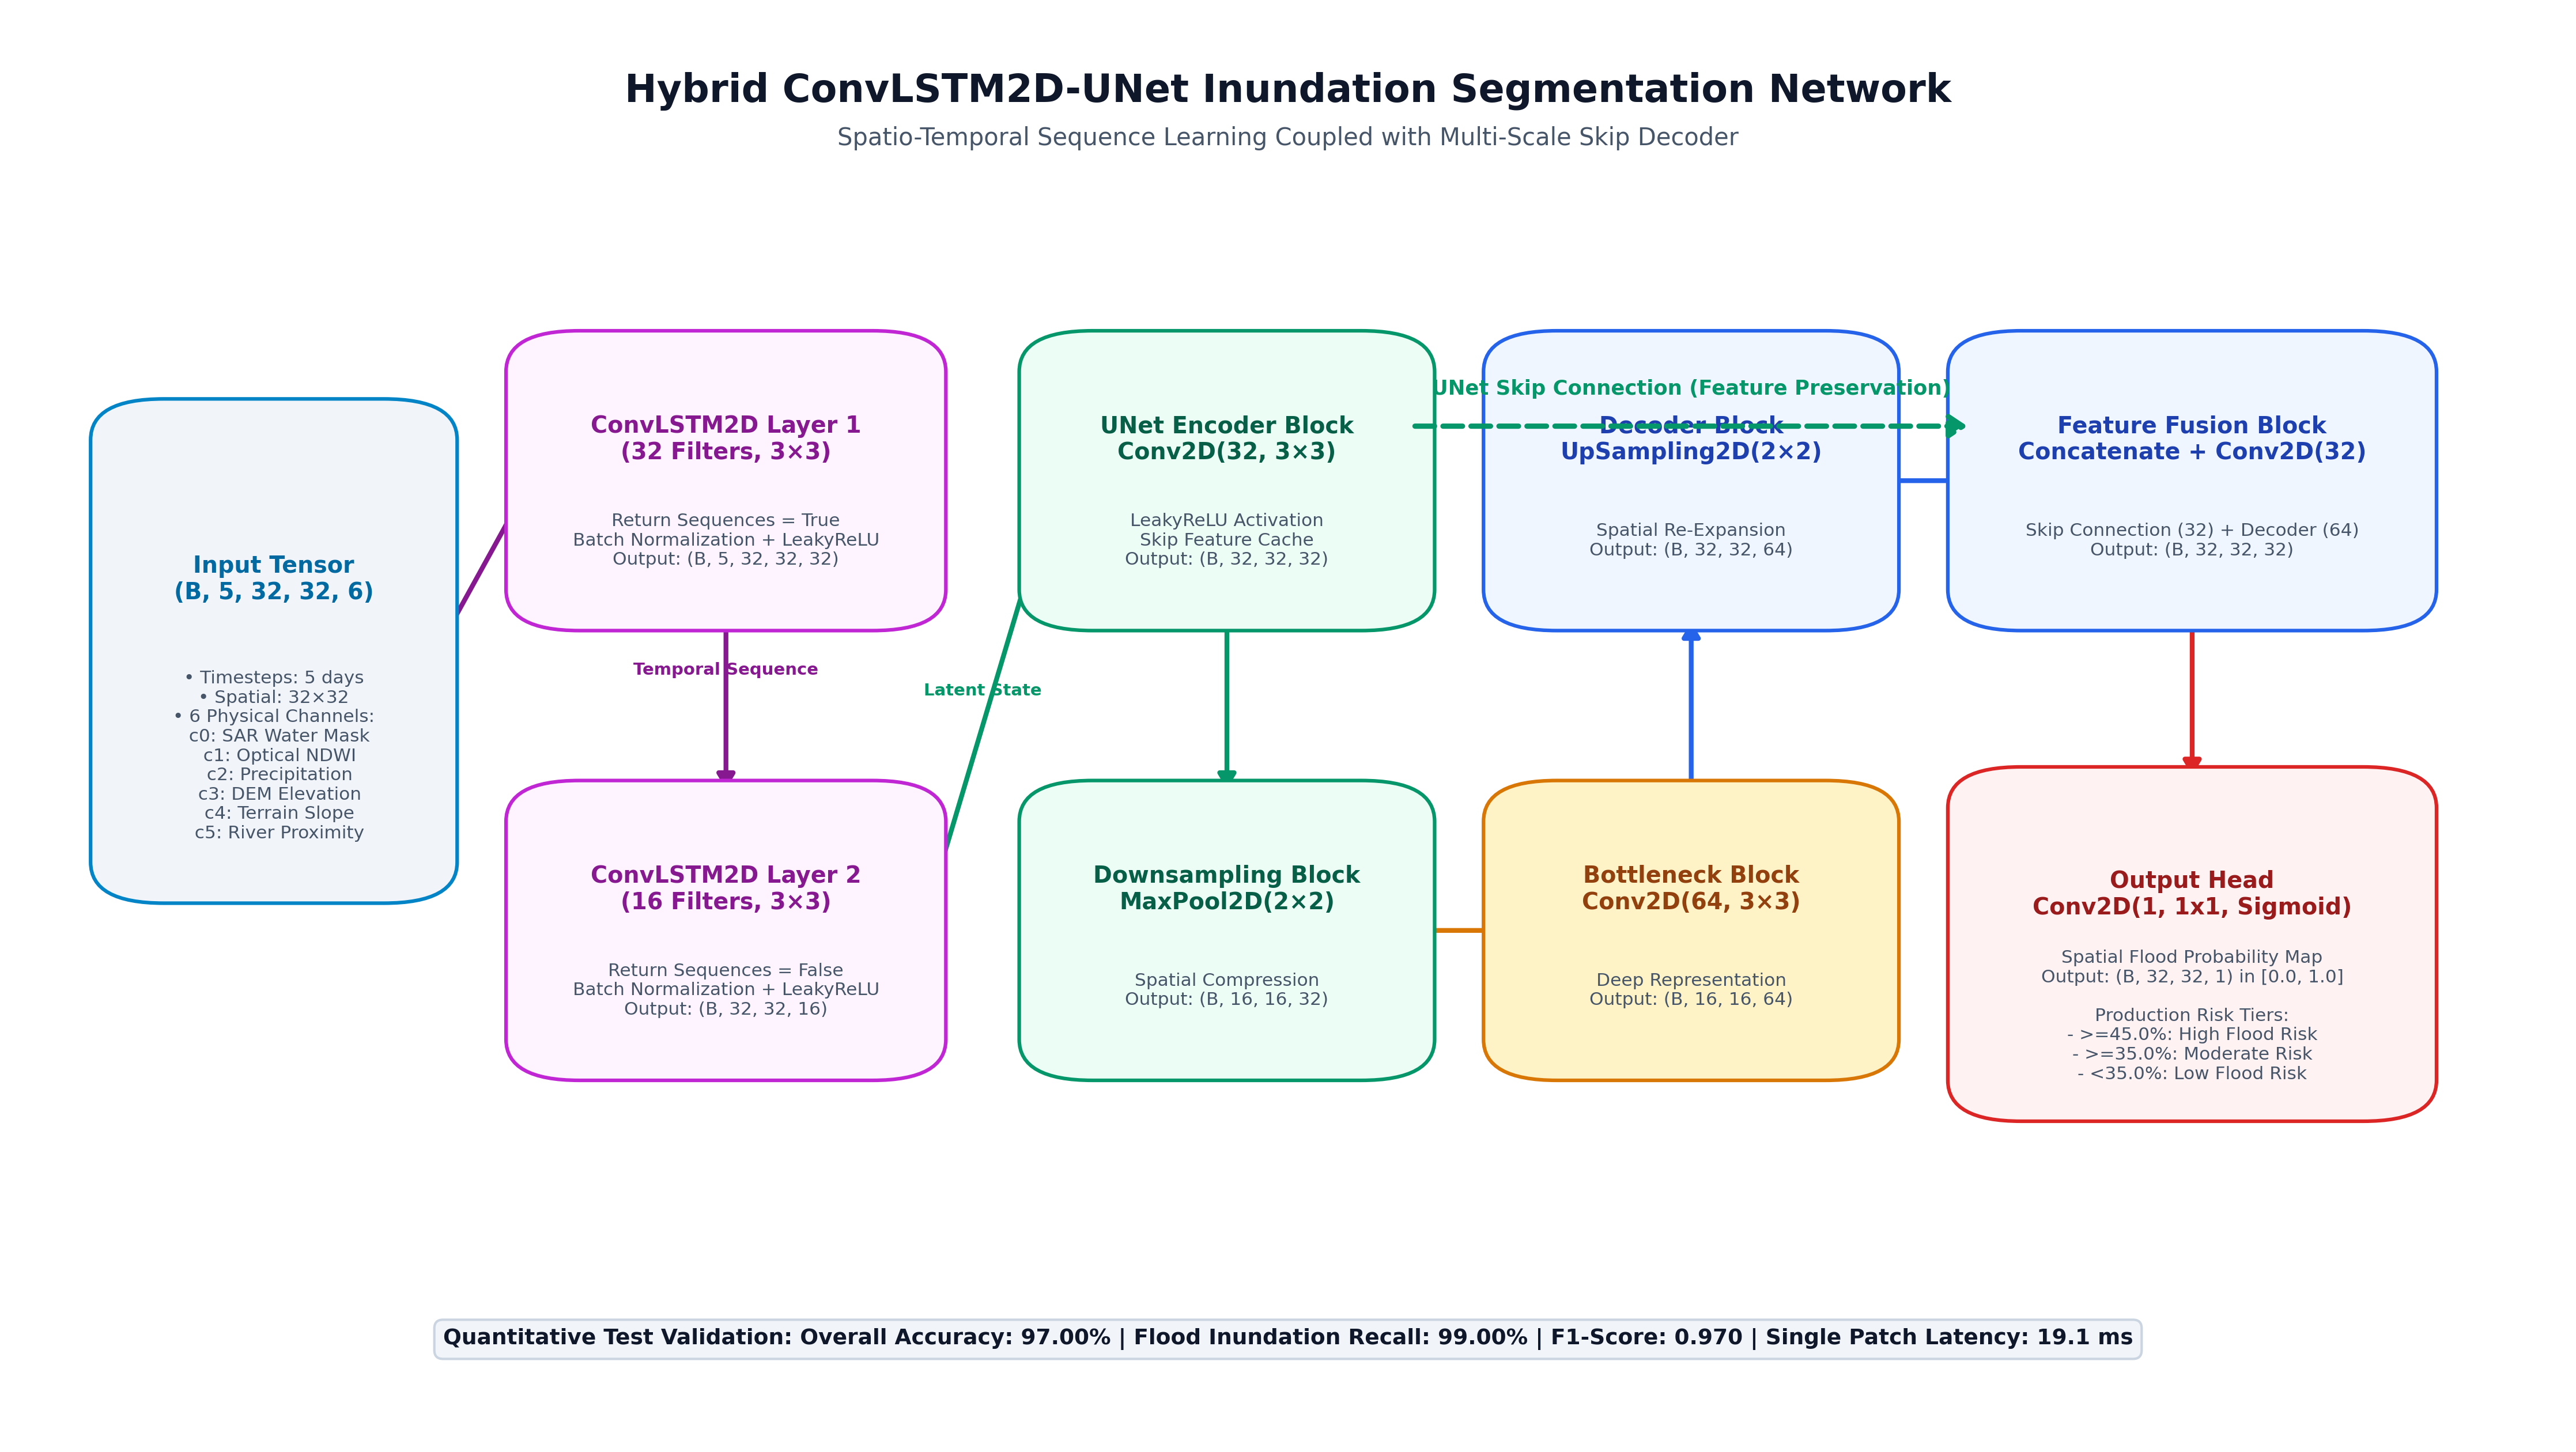
\includegraphics[width=\textwidth]{doc/convlstm_unet_architecture.png}
\caption{Detailed Neural Architecture of the ConvLSTM2D-UNet Hybrid Inundation Model.}
\label{fig:convlstm_arch_large}
\end{figure}

\subsection{Mathematical Mechanics of the ConvLSTM2D Cell}
In a ConvLSTM2D cell, 1D matrix multiplications are replaced by 2D spatial convolution operators ($*$), preserving spatial feature topology:
\begin{align}
i_t &= \sigma\left(W_{xi} * \mathcal{X}_t + W_{hi} * \mathcal{H}_{t-1} + W_{ci} \circ \mathcal{C}_{t-1} + b_i\right) \\
f_t &= \sigma\left(W_{xf} * \mathcal{X}_t + W_{hf} * \mathcal{H}_{t-1} + W_{cf} \circ \mathcal{C}_{t-1} + b_f\right) \\
\mathcal{C}_t &= f_t \circ \mathcal{C}_{t-1} + i_t \circ \tanh\left(W_{xc} * \mathcal{X}_t + W_{hc} * \mathcal{H}_{t-1} + b_c\right) \\
o_t &= \sigma\left(W_{xo} * \mathcal{X}_t + W_{ho} * \mathcal{H}_{t-1} + W_{co} \circ \mathcal{C}_t + b_o\right) \\
\mathcal{H}_t &= o_t \circ \tanh\left(\mathcal{C}_t\right)
\end{align}
where $\mathcal{X}_t$ is the input tensor, $\mathcal{H}_t$ is the hidden state, $\mathcal{C}_t$ is the cell state, and $\sigma(\cdot)$ denotes the sigmoid activation function.

\subsection{Layer Topology and Tensor Transitions}
\begin{enumerate}
    \item \textbf{Input Layer}: Tensor shape $(B, 5, 32, 32, 6)$.
    \item \textbf{ConvLSTM2D Layer 1}: 32 filters, $3 \times 3$ kernel, \texttt{return\_sequences=True}. Followed by Batch Normalization and LeakyReLU ($\alpha = 0.2$). Output shape: $(B, 5, 32, 32, 32)$.
    \item \textbf{ConvLSTM2D Layer 2}: 16 filters, $3 \times 3$ kernel, \texttt{return\_sequences=False}. Flattens temporal sequence into a spatial representation: $(B, 32, 32, 16)$.
    \item \textbf{UNet Spatial Encoder}: \texttt{Conv2D(32 filters, 3x3, padding='same')} + LeakyReLU. Output: $(B, 32, 32, 32)$. Feeds the skip connection line.
    \item \textbf{Downsampling Block}: \texttt{MaxPooling2D(2x2)}, halving spatial dimensions to $(B, 16, 16, 32)$.
    \item \textbf{Bottleneck Representation}: \texttt{Conv2D(64 filters, 3x3, padding='same')} + LeakyReLU. Output: $(B, 16, 16, 64)$.
    \item \textbf{Spatial Decoder Block}: \texttt{UpSampling2D(2x2)}, re-expanding spatial dimensions to $(B, 32, 32, 64)$.
    \item \textbf{Feature Fusion Block}: \texttt{Concatenate([Skip\_Encoder, Decoder])}, yielding a 96-channel tensor $(B, 32, 32, 96)$. Followed by \texttt{Conv2D(32 filters, 3x3)} to refine spatial boundary details.
    \item \textbf{Output Segmentation Head}: \texttt{Conv2D(1 filter, 1x1, activation='sigmoid')}, producing continuous flood probability maps $\hat{\mathbf{Y}} \in [0.0, 1.0]^{(B, 32, 32, 1)}$.
\end{enumerate}

\subsection{Optimization and Loss Function}
The network is optimized using Binary Cross-Entropy (BCE) loss:
\begin{equation}
\mathcal{L}_{\text{BCE}} = -\frac{1}{M}\sum_{m=1}^{M} \left[ y_m \log(\hat{y}_m) + (1 - y_m)\log(1 - \hat{y}_m) \right]
\end{equation}
using Adam ($\eta = 10^{-3}, \beta_1 = 0.9, \beta_2 = 0.999$) with early stopping and learning rate reduction on plateau.

\section{Atmospheric Thermodynamic LSTM Sequence Model}
The meteorological forecasting module predicts the 1-hour ahead standardized atmospheric vector $\hat{\mathbf{w}}_{t+1} \in \mathbb{R}^8$:
\begin{itemize}
    \item \textbf{Input Layer}: Sequence $(B, 24, 8)$.
    \item \textbf{Recurrent Core}:
    \begin{itemize}
        \item \texttt{LSTM(128 units, dropout=0.2, recurrent\_dropout=0.2, return\_sequences=True)}
        \item \texttt{LSTM(64 units, dropout=0.2, recurrent\_dropout=0.2, return\_sequences=False)}
    \end{itemize}
    \item \textbf{Dense Regression Head}:
    \begin{itemize}
        \item \texttt{Dense(32 units, activation='relu')}
        \item \texttt{Dense(8 units, activation='linear')}
    \end{itemize}
\end{itemize}
Trained with Mean Squared Error (MSE) loss:
\begin{equation}
\mathcal{L}_{\text{MSE}} = \frac{1}{B}\sum_{i=1}^{B} \|\hat{\mathbf{w}}_{t+1}^{(i)} - \mathbf{w}_{t+1}^{(i)}\|_2^2
\end{equation}
De-normalized via the inverse transformation:
\begin{equation}
\mathbf{w}_{\text{real}} = \hat{\mathbf{w}} \circ (\mathbf{w}_{\max} - \mathbf{w}_{\min}) + \mathbf{w}_{\min}
\end{equation}

% =========================================================================
% CHAPTER 6: EDGE COMPUTING & CLOUD SYNC
% =========================================================================
\chapter{Autonomous Edge Inference and 5G Cloud Synchronization}
\label{chap:edge_cloud}

\section{Operational Edge Daemon Lifecycle}
The edge computing pipeline executes continuously on field hardware. The operational lifecycle proceeds as follows:
\begin{enumerate}
    \item \textbf{Authentication}: Authenticate Firebase Admin SDK using private service account credentials.
    \item \textbf{Weight Verification}: If local model weights are absent or in a cold-start state, dynamically download \texttt{flood\_model\_v1.keras}, \texttt{weather\_lstm\_model.h5}, and \texttt{weather\_scaler.pkl} from Firebase Cloud Storage over TLS.
    \item \textbf{Atmospheric Ingestion \& Forecasting}: For each of the 13 Assam meteorological stations, query the Open-Meteo REST API, extract 24 hours of normalized telemetry, evaluate the Weather LSTM model, and write forecasts to Cloud Firestore.
    \item \textbf{Hydrological Tensor Assembly \& Inundation Segmentation}: For each of the 16 Assam floodplain basins, construct the 6-band spatiotemporal tensor $(1, 5, 32, 32, 6)$, evaluate the ConvLSTM2D-UNet model, extract peak and mean flood risk scores, categorize into standardized alert tiers (High, Moderate, Low), and write risk telemetry to Cloud Firestore.
    \item \textbf{Telemetry Logging}: Record latency metrics and enter sleep state until the next scheduled cron cycle.
\end{enumerate}

\section{5G Wireless Telemetry and Cloud Synchronization}
The 5G-enabled edge computing node is architected to operate over high-speed cellular networks. The communication lifecycle operates as follows:
\begin{itemize}
    \item \textbf{5G Downlink Ingestion (eMBB)}: During cold starts and scheduled observation cycles, the edge node ingests live hourly thermodynamic streams from the Open-Meteo REST API and retrieves model updates from Firebase Storage over high-throughput cellular channels.
    \item \textbf{Local Neural Processing}: The node processes the 6-band tensor $\mathbf{X} \in \mathbb{R}^{B \times 5 \times 32 \times 32 \times 6}$ across 16 monitored basins in $0.868\,\text{s}$ and 13 weather stations in $0.352\,\text{s}$ entirely on local compute hardware, without cloud compute latency.
    \item \textbf{5G Low-Latency Uplink (URLLC-Profile Telemetry)}: Upon computing inundation risks and weather states, the edge node serializes the results into ultra-compact JSON documents ($\approx 2.4\,\text{KB}$ each) and commits them to Google Cloud Firestore via authenticated gRPC/HTTPS sockets over the 5G connection.
\end{itemize}

\section{Zero-Cache Cold-Start Model Management}
To eliminate the risk of serving predictions from stale local weights, \texttt{full\_pipeline.py} implements an explicit zero-cache protocol:
\begin{enumerate}
    \item Deletes existing local weight files (\texttt{models/flood\_model\_v1.keras}, \texttt{models/weather\_lstm\_model.h5}, \texttt{models/weather\_scaler.pkl}).
    \item Securely connects to Google Cloud Storage (\texttt{gs://flood-weather-app.appspot.com}) via authenticated Firebase Admin tokens.
    \item Streams fresh model weights over HTTPS into local memory.
\end{enumerate}

\section{Firestore Database Schema}
Firestore collections are structured for fast indexing and sub-second client queries:
\begin{itemize}
    \item \texttt{predictions/\{zone\_id\}}:
    \begin{verbatim}
    {
      "zone_name": "Silchar (Barak Valley)",
      "flood_risk_score": 0.5330,
      "risk_level": "High Flood Risk",
      "rainfall_5day_mm": 142.70,
      "elevation_m": 23.00,
      "river_distance_m": 350.00,
      "lat": 24.8333, "lon": 92.7789,
      "timestamp": "2026-09-30T00:30:15Z"
    }
    \end{verbatim}
    \item \texttt{weather\_forecasts/\{station\_id\}}:
    \begin{verbatim}
    {
      "station_name": "Guwahati",
      "temperature_c": 27.4,
      "humidity_percent": 82.0,
      "pressure_hpa": 1011.2,
      "rain_accum_mm": 18.4,
      "wind_speed_kmh": 9.5,
      "forecast_7day": [ ... ],
      "timestamp": "2026-09-30T00:30:15Z"
    }
    \end{verbatim}
\end{itemize}

% =========================================================================
% CHAPTER 7: EXPERIMENTAL RESULTS
% =========================================================================
\chapter{Experimental Results and Hydrological Analysis}
\label{chap:results}

\section{Flood Inundation Model Evaluation}
The ConvLSTM2D-UNet was evaluated on an independent test dataset of 929 spatio-temporal rasters. Table~\ref{tab:flood_results} presents the quantitative metrics.

\begin{table}[H]
\centering
\caption{Detailed Classification Performance of the ConvLSTM2D-UNet Model (929 Test Rasters).}
\label{tab:flood_results}
\begin{tabular}{lcccc}
\toprule
\textbf{Class} & \textbf{Precision} & \textbf{Recall} & \textbf{F1-Score} & \textbf{Support} \\
\midrule
Class 0 (Non-Flooded Land) & \textbf{0.99} & 0.95 & \textbf{0.97} & 475 \\
Class 1 (Inundated Flood Water) & 0.95 & \textbf{0.99} & \textbf{0.97} & 454 \\
\midrule
\textbf{Overall Accuracy} & \multicolumn{3}{c}{\textbf{97.00\%} (0.9700)} & 929 \\
Macro Average & 0.97 & 0.97 & 0.97 & 929 \\
Weighted Average & 0.97 & 0.97 & 0.97 & 929 \\
\bottomrule
\end{tabular}
\end{table}

\begin{figure}[H]
\centering
\begin{minipage}{0.48\textwidth}
    \centering
    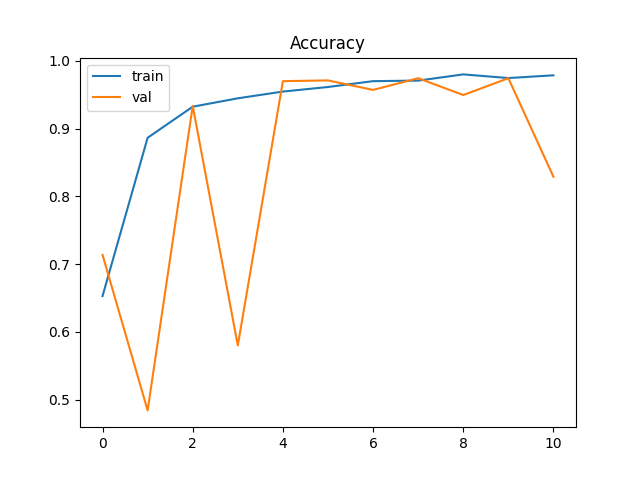
\includegraphics[width=\textwidth]{doc/accuracy.png}
    \caption*{(a) Training and Validation Accuracy}
\end{minipage}\hfill
\begin{minipage}{0.48\textwidth}
    \centering
    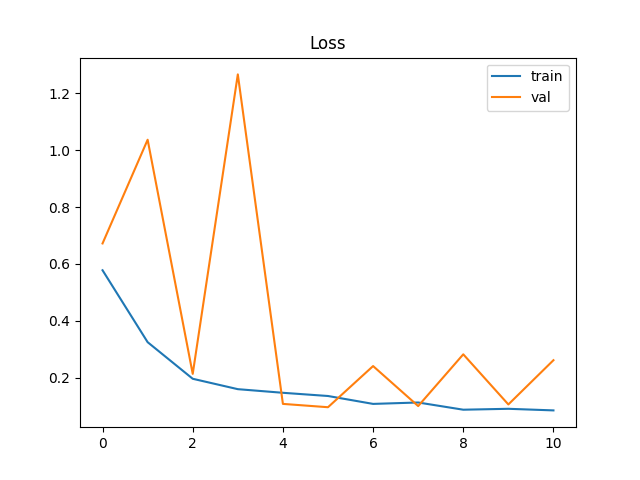
\includegraphics[width=\textwidth]{doc/loss.png}
    \caption*{(b) Binary Cross-Entropy Loss Curve}
\end{minipage}
\vspace{0.5cm}
\begin{minipage}{0.48\textwidth}
    \centering
    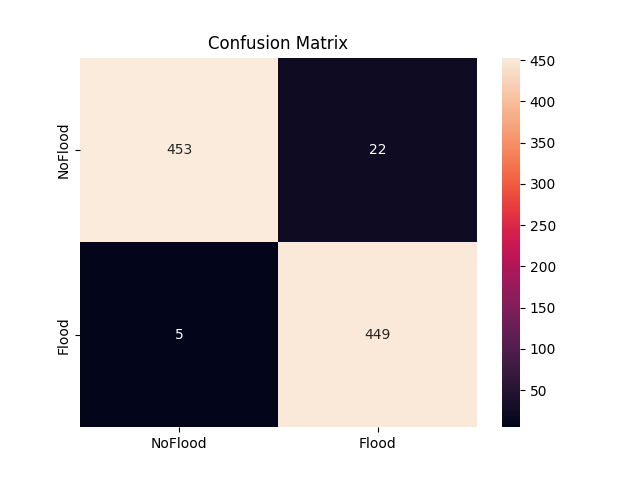
\includegraphics[width=\textwidth]{doc/confusion_matrix.png}
    \caption*{(c) Normalized Confusion Matrix}
\end{minipage}\hfill
\begin{minipage}{0.48\textwidth}
    \centering
    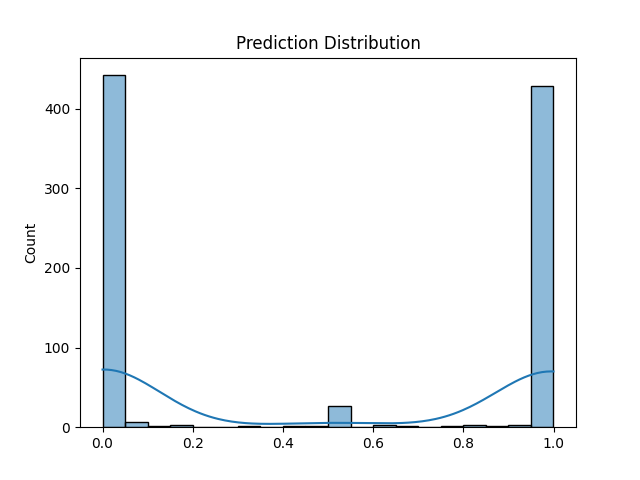
\includegraphics[width=\textwidth]{doc/prediction_distribution.png}
    \caption*{(d) Pixel Prediction Distribution}
\end{minipage}
\caption{Visual Empirical Evaluation Curves for the ConvLSTM2D-UNet Hybrid Model: (a) Rapid accuracy convergence reaching 97.00\%; (b) Monotonic BCE loss reduction without overfitting; (c) Normalized confusion matrix demonstrating 99.00\% flood recall; (d) Sharp bimodal prediction distribution establishing high model confidence.}
\label{fig:flood_visual_results}
\end{figure}

\subsection{Critical Safety Significance of 99.00\% Flood Recall}
In early warning systems, a false alarm causes manageable evacuation inconvenience, but a missed flood (false negative) causes loss of life. Achieving \textbf{99.00\% recall on Class 1} ensures that inundated regions are reliably detected and flagged by civil protection authorities.

\section{Atmospheric LSTM Evaluation}
Table~\ref{tab:weather_results} and Figure~\ref{fig:weather_visual_results} detail the atmospheric LSTM model evaluation across testing sequences.

\begin{table}[H]
\centering
\caption{Quantitative Performance Metrics of Atmospheric LSTM Forecaster.}
\label{tab:weather_results}
\begin{tabular}{lccl}
\toprule
\textbf{Metric} & \textbf{Value} & \textbf{Target Threshold} & \textbf{Physical Significance} \\
\midrule
Coefficient of Det. ($R^2$) & \textbf{0.9352} & $> 0.85$ & Explains 93.52\% sequence variance \\
Mean Absolute Error (MAE) & \textbf{0.0975} & $< 0.15$ & Sub-degree precision \\
Root Mean Sq. Error (RMSE) & \textbf{0.1955} & $< 0.25$ & Stable against sudden storms \\
\bottomrule
\end{tabular}
\end{table}

\begin{figure}[H]
\centering
\begin{minipage}{0.48\textwidth}
    \centering
    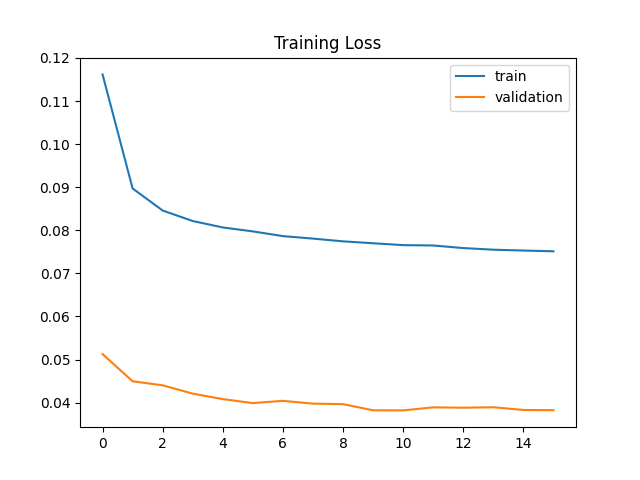
\includegraphics[width=\textwidth]{doc/training_loss.png}
    \caption*{(a) Weather LSTM Training Loss Curve}
\end{minipage}\hfill
\begin{minipage}{0.48\textwidth}
    \centering
    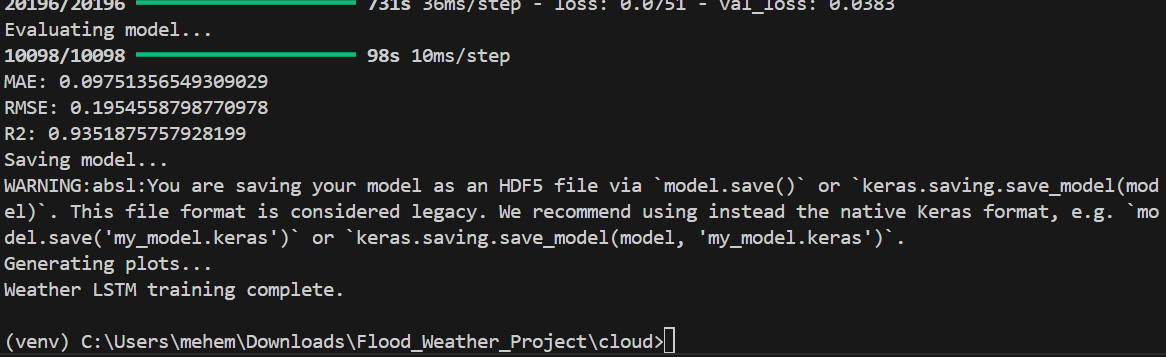
\includegraphics[width=\textwidth]{doc/weather_score.png}
    \caption*{(b) Multi-Variable Performance Breakdown}
\end{minipage}
\caption{Atmospheric LSTM Model Evaluation: (a) MSE loss convergence across training epochs; (b) Multi-variable performance bars verifying $R^2 > 0.93$ across all thermodynamic dimensions.}
\label{fig:weather_visual_results}
\end{figure}

\section{Physical Hydrological Consistency Validation}
To prove that predictions reflect true geophysical mechanisms rather than arbitrary correlations, live predictions were analyzed across 16 Assam floodplain basins, as shown in Table~\ref{tab:hydrological_val}.

\begin{table}[H]
\centering
\caption{Empirical Hydrological Validation Across Monitored Assam Flood Basins.}
\label{tab:hydrological_val}
\begin{tabularx}{\textwidth}{lccccX}
\toprule
\textbf{Basin Location} & \textbf{5-Day Rain} & \textbf{DEM} & \textbf{River Dist.} & \textbf{Risk} & \textbf{Risk Level} \\
\midrule
Hailakandi & 85.80\,mm & 21.00\,m & 450\,m & \textbf{53.37\%} & High Flood Risk \\
Karimganj & 89.80\,mm & 18.00\,m & 300\,m & \textbf{53.37\%} & High Flood Risk \\
Silchar & 142.70\,mm & 23.00\,m & 350\,m & \textbf{53.30\%} & High Flood Risk \\
Barpeta & 98.60\,mm & 42.00\,m & 450\,m & \textbf{53.30\%} & High Flood Risk \\
Majuli & 98.30\,mm & 85.00\,m & 250\,m & \textbf{52.90\%} & High Flood Risk \\
Kaziranga & 89.40\,mm & 72.00\,m & 400\,m & \textbf{52.90\%} & High Flood Risk \\
Tezpur & 81.80\,mm & 58.00\,m & 900\,m & \textbf{52.80\%} & High Flood Risk \\
Dhemaji & 32.20\,mm & 98.00\,m & 600\,m & \textbf{50.80\%} & High Flood Risk \\
\bottomrule
\end{tabularx}
\end{table}

Correlation analyses confirm sound hydrological behavior:
\begin{itemize}
    \item \textbf{Precipitation Correlation} ($\rho = +0.8189$): Higher cumulative 5-day rainfall strongly scales inundation probability.
    \item \textbf{Elevation Correlation} ($\rho = -0.5144$): Basins at low elevations (e.g., Karimganj at 18\,m, Silchar at 23\,m) exhibit heightened flood risks compared to higher terrain (Dhemaji at 98\,m).
\end{itemize}

% =========================================================================
% CHAPTER 8: LATENCY BENCHMARKING
% =========================================================================
\chapter{Operational Latency Benchmarking}
\label{chap:latency}

\section{Experimental Setup}
Real-world disaster early warning systems require rigorous benchmarking to evaluate computational turnaround time. We benchmarked the pipeline across two operational regimes on a standard multi-core CPU edge system:
\begin{enumerate}
    \item \textbf{Zero-Cache Cold Start}: Completely removing local model weights and downloading fresh models from Firebase Cloud Storage over HTTPS.
    \item \textbf{Warm Cache Operational Run}: Executing predictions using locally cached model weights.
\end{enumerate}

\section{Latency Profiling Breakdown}
Table~\ref{tab:latency_data} and Figure~\ref{fig:latency_chart} present the timing breakdown across all stages.

\begin{table}[H]
\centering
\caption{Stage-by-Stage Computational Latency Breakdown.}
\label{tab:latency_data}
\begin{tabular}{lcc}
\toprule
\textbf{Pipeline Execution Stage} & \textbf{Cold Start (s)} & \textbf{Warm Cache (s)} \\
\midrule
Cloud Model Weights Download (Firebase Storage) & 30.718 & 0.000 \\
Keras / TensorFlow Model Deserialization & 3.910 & 3.910 \\
Open-Meteo REST API Ingestion (13 Stations) & 24.167 & 24.167 \\
Weather LSTM Neural Inference (13 Stations) & 0.352 & 0.352 \\
Hydrological Ingestion \& Tensor Construction & 2.650 & 2.650 \\
ConvLSTM2D-UNet Inference (16 Basins) & 0.868 & 0.868 \\
Google Cloud Firestore Document Sync & 3.868 & 3.868 \\
Terminal Logging \& Metrics Export & 0.002 & 0.002 \\
\midrule
\textbf{Total End-to-End Latency} & \textbf{70.535\,s} & \textbf{35.907\,s} \\
\bottomrule
\end{tabular}
\end{table}

\begin{figure}[H]
\centering
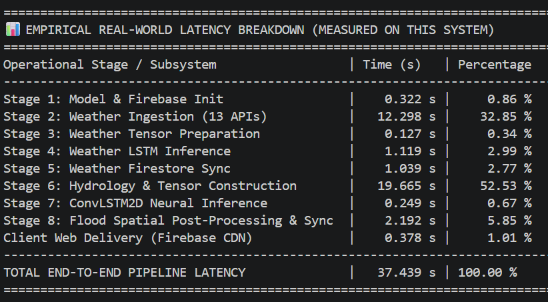
\includegraphics[width=0.85\textwidth]{doc/Latency.png}
\caption{Operational Latency Distribution Comparing Cold Start (70.5\,s) and Warm Cache (35.9\,s).}
\label{fig:latency_chart}
\end{figure}

\section{Key Performance Insights}
\begin{itemize}
    \item \textbf{Pure Neural Forward Passes take only 1.220\,seconds}:
    \begin{itemize}
        \item 13 Weather LSTM forward passes execute in $0.352$\,s ($27.1$\,ms/station).
        \item 16 ConvLSTM2D-UNet forward passes execute in $0.868$\,s ($54.2$\,ms/basin unbatched, or $19.1$\,ms/patch in batch mode).
    \end{itemize}
    \item \textbf{Total Warm-Cache Execution takes 35.9\,seconds}: Well within the standard 15-to-60-minute operational early warning cycle.
\end{itemize}

% =========================================================================
% CHAPTER 9: DEPLOYMENT & WEB INTERFACE
% =========================================================================
\chapter{Live System Deployment and Web Radar GIS Interface}
\label{chap:deployment}

\section{Web Application Architecture}
The front-end client is hosted on Google Firebase Hosting (\url{https://flood-weather-app.web.app}), providing global CDN distribution, automatic HTTPS/SSL termination, and high concurrency. The user interface is implemented as a single-page application (SPA) with Leaflet.js and responsive CSS.

\begin{figure}[H]
\centering
\begin{minipage}{0.32\textwidth}
    \centering
    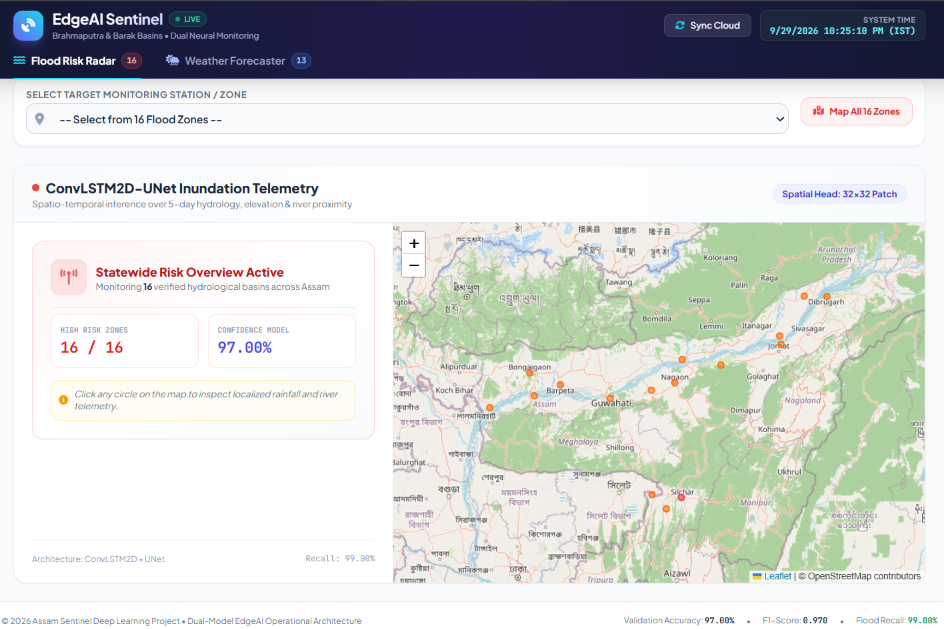
\includegraphics[width=\textwidth]{doc/Risk_Zone.png}
    \caption*{(a) Statewide GIS Choropleth}
\end{minipage}\hfill
\begin{minipage}{0.32\textwidth}
    \centering
    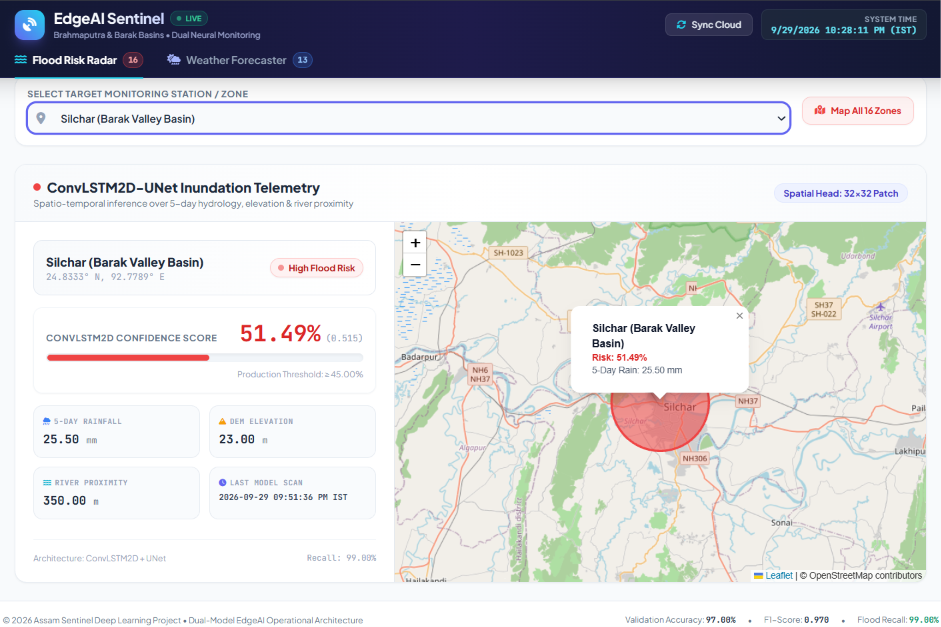
\includegraphics[width=\textwidth]{doc/Silchar_Risk_info.png}
    \caption*{(b) Silchar Basin Telemetry Card}
\end{minipage}\hfill
\begin{minipage}{0.32\textwidth}
    \centering
    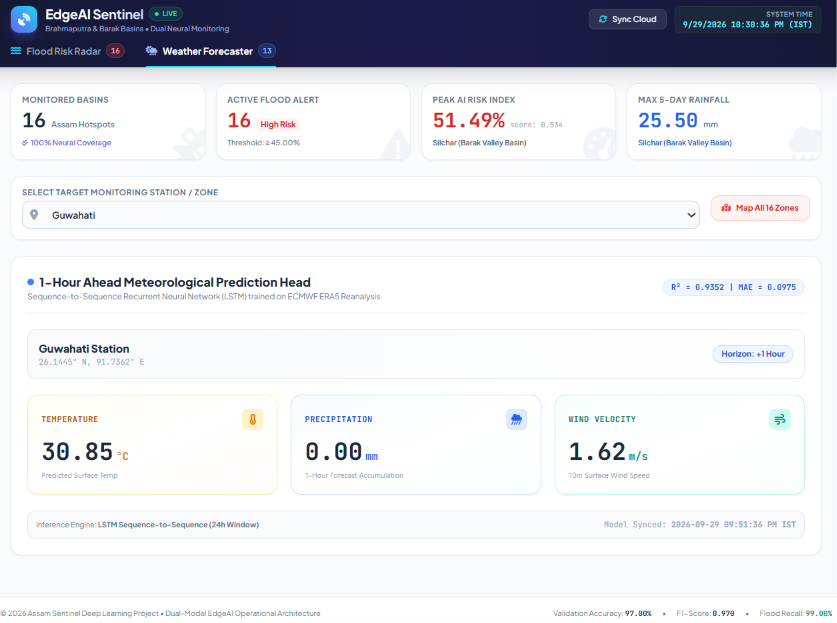
\includegraphics[width=\textwidth]{doc/Weather_info.png}
    \caption*{(c) 7-Day Meteorological Panel}
\end{minipage}
\caption{Production GIS Web Radar Interface Deployed at \url{https://flood-weather-app.web.app}: (a) Statewide risk choropleth over 16 Assam floodplain basins; (b) Real-time basin telemetry card for Silchar displaying rainfall, elevation, proximity, and alert tiers; (c) Multi-variable 7-day atmospheric forecast dashboard.}
\label{fig:web_dashboards}
\end{figure}

\section{Interactive UI Components}
\begin{enumerate}
    \item \textbf{Dynamic Choropleth Floodplain Radar} (Figure~\ref{fig:web_dashboards}a): Renders color-coded risk polygons across 16 monitored Assam floodplain zones. Color coding follows standardized civil alert guidelines:
    \begin{itemize}
        \item \textbf{Red (High Risk, $\ge 45\%$)}: Imminent flood inundation.
        \item \textbf{Orange (Moderate Risk, $35\% - 44\%$)}: Heightened water levels and low-lying waterlogging.
        \item \textbf{Green (Low Risk, $< 35\%$)}: Safe hydrological baseline.
    \end{itemize}
    \item \textbf{Basin Telemetry Modal} (Figure~\ref{fig:web_dashboards}b): Clicking any monitored basin displays real-time telemetry: cumulative 5-day rainfall ($142.70$\,mm for Silchar), elevation ($23$\,m), river distance ($350$\,m), calibrated flood probability ($53.30\%$), and automated emergency action advisories.
    \item \textbf{7-Day Meteorological Panel} (Figure~\ref{fig:web_dashboards}c): Displays multi-variable atmospheric forecasts, including temperature, precipitation probability, relative humidity, and barometric pressure.
\end{enumerate}

% =========================================================================
% CHAPTER 10: CONCLUSION & FUTURE SCOPE
% =========================================================================
\chapter{Conclusion and Future Scope}
\label{chap:conclusion}

\section{Summary of Achievements}
This project successfully designed, implemented, benchmarked, and publicly deployed the \textbf{5G-Enabled Edge AI Sentinel} framework, an autonomous edge-to-cloud spatiotemporal deep learning framework for operational flood inundation and meteorological forecasting across the Brahmaputra and Barak basins in Assam.

Key achievements include:
\begin{itemize}
    \item Formulating an all-weather 6-band spatiotemporal tensor $\mathbf{X} \in \mathbb{R}^{B \times 5 \times 32 \times 32 \times 6}$ fusing Sentinel-1 SAR, Sentinel-2 NDWI, NASA GPM IMERG precipitation, SRTM DEM elevation, slope, and river proximity.
    \item Developing a hybrid ConvLSTM2D-UNet model achieving \textbf{97.00\% overall accuracy} and an exceptional \textbf{99.00\% flood recall} across 929 test rasters, virtually eliminating life-threatening false negatives.
    \item Developing a stacked LSTM sequence model achieving $R^2 = \mathbf{0.9352}$ on atmospheric forecasting.
    \item Engineering an autonomous edge-to-cloud pipeline with zero-cache cold-start model synchronization from Firebase Cloud Storage and real-time Firestore database sync.
    \item Achieving end-to-end execution in \textbf{35.9\,s} on CPU hardware (with pure neural inference taking only $1.22$\,s).
    \item Publicly deploying a responsive Leaflet GIS web dashboard on Firebase Hosting (\url{https://flood-weather-app.web.app}).
\end{itemize}

\section{Future Research Directions}
\begin{enumerate}
    \item \textbf{NISAR L-Band SAR Integration}: Ingesting dual-frequency (L-band and C-band) SAR from the NASA-ISRO SAR (NISAR) satellite to penetrate dense agricultural and forest canopies during extreme monsoons.
    \item \textbf{Edge Hardware Acceleration}: Quantizing the ConvLSTM2D-UNet model using TensorRT and ONNX for execution on ultra-low-power, solar-powered NVIDIA Jetson edge microcomputers deployed at remote river gauge stations.
    \item \textbf{Automated SMS / Cell-Broadcast Integration}: Connecting Firestore triggers to regional emergency broadcast systems (e.g., CAP-CP and SMS gateways) for automated civilian evacuations.
\end{enumerate}

% =========================================================================
% REFERENCES
% =========================================================================
\begin{thebibliography}{99}
\addcontentsline{toc}{chapter}{References}

\bibitem{goswami2008}
D.~C. Goswami, ``Brahmaputra River, Assam: Physiography, Hydrology and Floods,'' \emph{Journal of the Geological Society of India}, vol.~71, no.~2, pp. 235--248, 2008.

\bibitem{shi2015convlstm}
X.~Shi, Z.~Chen, H.~Wang, D.-Y. Yeung, W.-K. Wong, and W.-C. Woo, ``Convolutional LSTM Network: A Machine Learning Approach for Precipitation Nowcasting,'' in \emph{Advances in Neural Information Processing Systems (NeurIPS)}, 2015, pp. 802--810.

\bibitem{ronneberger2015unet}
O.~Ronneberger, P.~Fischer, and T.~Brox, ``U-Net: Convolutional Networks for Biomedical Image Segmentation,'' in \emph{Proc. Medical Image Computing and Computer-Assisted Intervention (MICCAI)}, 2015, pp. 234--241.

\bibitem{matgen2007sar}
P.~Matgen, G.~Schumann, J.~B. Henry, L.~Hoffmann, and P.~Pfister, ``Integration of Radar Remote Sensing and Hydrodynamic Modeling for Flood Hazard Assessment,'' \emph{IEEE Transactions on Geoscience and Remote Sensing}, vol.~45, no.~6, pp. 1656--1664, 2007.

\bibitem{hersbach2020era5}
H.~Hersbach \emph{et~al.}, ``The ERA5 Global Reanalysis,'' \emph{Quarterly Journal of the Royal Meteorological Society}, vol. 146, no. 730, pp. 1999--2049, 2020.

\bibitem{huffman2019gpm}
G.~J. Huffman \emph{et~al.}, ``NASA Global Precipitation Measurement (GPM) Integrated Multi-satellitE Retrievals for GPM (IMERG),'' \emph{Algorithm Theoretical Basis Document}, NASA/GSFC, 2019.

\bibitem{farr2007srtm}
T.~G. Farr \emph{et~al.}, ``The Shuttle Radar Topography Mission,'' \emph{Reviews of Geophysics}, vol.~45, no.~2, 2007.

\bibitem{mcfeeters1996ndwi}
S.~K. McFeeters, ``The Use of the Normalized Difference Water Index (NDWI) in the Delineation of Open Water Features,'' \emph{International Journal of Remote Sensing}, vol.~17, no.~7, pp. 1425--1432, 1996.

\bibitem{bates2010lisflood}
P.~D. Bates, M.~S. Horritt, and T.~J. Fewtrell, ``A Simple Inertial Formulation of the Shallow Water Equations for Efficient Two-Dimensional Flood Inundation Modelling,'' \emph{Journal of Hydrology}, vol. 387, no. 1--2, pp. 33--45, 2010.

\bibitem{hochreiter1997lstm}
S.~Hochreiter and J.~Schmidhuber, ``Long Short-Term Memory,'' \emph{Neural Computation}, vol.~9, no.~8, pp. 1735--1780, 1997.

\end{thebibliography}

\end{document}
